\chapter{Tests in Metamodel Fitting}

The fitting of SMT metamodels is tested on a pair 
of low-fidelity models that are used as conceptual level 
estimate of the wing weight of an aircraft. The testing phase 
initiates by creating a DoE design w.r.t. a semi-arbitrarily 
imposed lower and upper bound for each design variable. This DoE 
design consists of $n_{t}$ training data, which are subsequently 
evaluated on the problem-specific low-fidelity model, i.e. the 
exact evaluation model. The resulting $n_{t}$ $(\vec{β},\vec{f}
(\vec{β})$ pairs are used for the training of a selected surrogate 
model. After the training process has been completed, a new set of 
sample points is selected from the design space via the use of DoE 
techniques. These are called validation points, are equal in number 
to training points, i.e. $n_{t} \!= \!n_{val} \!= \!40$ and are 
used to validate the accuracy of the trained metamodel. 
Validation points are evaluated using both the exact 
evaluation model and the trained metamodel resulting in 
$\mathbf{F}$ and $\hat{\mathbf{F}}$ values, respectively. The 
deviation between these values for the $n_{t}$ training data is 
calculated by the use of NRMSE, which serves as a metric for 
metamodel accuracy. The computations have been performed on a 
i7-9750H, 2.60 GHz CPU.
\vfill

\section{3 design variable aircraft wing equation}
\label{appendix:pseudo_aircraft}
The quality of each metamodel is tested in a simplistic 3 
design variable wing weight equation that is used for the 
conceptual design of light, low performance aircrafts. This 
equation applies to cantilever wings and includes the weight 
of wing tip and flight control surfaces, i.e. ailerons, while
it excludes fuel tank weight, the effect of sweep angle 
and spar flight loads from wing and fuselage. The wing 
weight is determined from the following 
equation\cite{wing_weight}:

\begin{equation}
W_{wing} = 0.0467W_{TO}^{0.397}S^{0.397}N_{z}^{0.360}
AR^{1.712}
\end{equation}
\\[-0.3cm]
where $W_{TO}$ is the aircraft take-off weight, $N_{z}$ 
the ultimate load factor, $S$ the wing area and $AR$ the 
wing aspect ratio. The search of a low-performance, light 
utility aircraft with maximum speed $V_{flight} < 200$ 
$kn$ resulted in the selection of Evektor VUT1OO-131i 
Cobra\cite{Evektor}. The aforementioned aircraft is used 
as a template and its design values are set as a baseline 
for the range of each design variable in the previous 
equation.

\begin{table}[h!]
\centering
\scalebox{0.86}{%
%\rowcolors{1}{gray!30!}{white!50!gray!10}
\begin{tabular}[c]{|p{2.3cm}|p{2.3cm}|p{2.3cm}|p{2.3cm}|}
\toprule
\multicolumn{4}{|c|}{\cellcolor{gray!30!}
\textbf{VUT1OO-131i Cobra}} 
\\
\midrule 
$\mathbf{MTOW}$ [lb] & $\mathbf{S}$ [$ft^2$] & 
$\mathbf{N_{z}}$ & $\mathbf{AR}$ \\
\hline
3,197 & 141.1 & 3.8 & 8.4 \\
\bottomrule
\end{tabular}
}
\caption{Design values for VUT100-131i Cobra}
\end{table}

\newpage
%----------------------------------------------------------


By making the assumption that take-off weight is a
constant parameter arbitrarily set equal to $W_{TO} = 
2,500 \hspace{2mm} lb$, then the previous equation can be 
restated as such:
\begin{equation}\label{pseudo_aircraft}
W_{wing} = 1.043S^{0.397}N_{z}^{0.360}
AR^{1.712}
\end{equation}
\\[-0.3cm]
The design space under study now consists of three 
independent design variables ${S,N_{z},AR}$ that define 
the design variable vector $\vec{β} = [S,N_{z},AR]$. 
The range of each design variable is set arbitrarily as 
such:
\begin{itemize}
\itemsep0em 
\item  $120 < S < 170$
\item $2 < N_{z} < 6$
\item $6 < AR < 11$
\end{itemize}
 
The deviation between the predicted and the exact model 
value for $n_{val}$ validation points is 
subsequently depicted in the following figures: 
 
\newpage
%-----------------------------------------------------------


\section{8 design variable aircraft wing equation}
With the testing of the first objective function now
complete, the ability of SMT metamodels to handle high-dimensional 
problems is still in question. For this reason, the software's 
capabilities will now be tested in an objective function consisting 
of 8 design variables. An increase in the number of design 
variables is expected to increase the complexity of the problem and 
therefore the computational cost. Consequently, an increase in 
design variables is a good metric of the software responsiveness to 
problems of higher dimensionality.   

The second weight equation is used for the conceptual 
design of cargo/transport aircrafts. This equation 
accounts for the effect of sweep angle and 
excludes fuel tank weight and spar flight loads from wing 
and fuselage. The wing weight is determined from the 
following equation \cite{wing_weight}:

\begin{equation} \label{aircraft2}
W_{wing} = 0.0051 (W_{dg}N_{z})^{0.557} S^{0.649} 
AR^{0.0035} \left( \dfrac{t}{c} \right)_{root}^{-0.4} 
(1 + λ)^{0.1} (cosΛ)^{-1} S_{c}^{0.1}
\end{equation}
\\
where $W_{dg}$ is the flight design gross weight, $N_{z}$ 
the ultimate load factor, $S$ is the wing area, $AR$ the 
aspect ratio, $λ_{r}$ the taper ratio, $Λ$ the 
quarter-chord sweep, $(t/c)$ the airfoil thickness to cord 
ratio at the root of the wing and $S_{c}$ flight control 
surface area. A search for a cargo aircraft resulted in 
the selection of Airbus A400M Atlas. Its design values
are presented in the following table: 

\begin{table}[h!]
\centering
\scalebox{0.9}{%
%\rowcolors{1}{gray!30!}{white!50!gray!10}
\begin{tabular}[c]{|p{2.3cm}|p{2.3cm}|p{2.3cm}|}
\toprule
\multicolumn{3}{|c|}{\cellcolor{gray!30!} \textbf{A400M 
Atlas}} \\
\midrule
$\bm{W_{dg}}$ & 264555 & $[lb]$ \\
$\mathbf{N_{z}}$ & -  & - \\
$\mathbf{S}$ & 2384 & [$ft^2$] \\
$\mathbf{AR}$ & 8.1 & - \\
$\mathbf{(t/c)_{root}}$ & - & -  \\
$\mathbf{λ_{r}}$ & - & - \\
$\mathbf{Λ}$ & 15 & [degrees] \\
$\mathbf{S_{c}}$ & 867 & $[ft^{2}]$ \\
\bottomrule
\end{tabular}
}
\caption{Airbus A400M Atlas design values}
\end{table} 

where the constrictions for each variable involved are:
\begin{itemize}
\itemsep0em
\item $220000 \leq W_{dg} \leq 280000$
\item $ 2.5 \leq N_{z} \leq 10 $ 
\item $2000 \leq S \leq 3000$
\item $6 \leq AR \leq 10$
\item $ 0.08 \leq t_{c} \leq 0.18$
\item $0.5 \leq \lambda \leq 1$
\item $ -20 \leq \Lambda \leq 20$
\item $400 \leq S_{c} \leq 2000$


\end{itemize} 

\newpage
%--------------------------------------------------------

\section{Optimal construction method }
\label{appendix:constr_crit} 

The main parameter affecting the quality of an LHD is the
construction criterion, denoted as $criterion$ in Python. 
The fitting of the trained metamodel is used as a metric for the 
quality of the profuced design. The parametric analysis 
is applied on eq. \ref{aircraft2} that consists of 8 objective 
variables. The surrogate model utilized here is KPLS with 
regression model (denoted as $poly$) and correlation function 
(denoted as $corr$) set to their default values, i.e 
'constant' and '$squar\_exp$' respectively. The design space is 
reduced to $n\_comp = 3$ dimensions. The constructed designs 
consist of $n_{doe} \!= \! 25$ sample points.
 
\begin{table}[h]
\centering
\scalebox{0.86}{%
%\rowcolors{2}{gray!30!}{white!50!gray!10}
\begin{tabular}[c]{ |p{2cm}||p{2cm}|p{2cm}|p{2cm}|p{2cm}|}
\toprule 
\multicolumn{5}{|c|}{\cellcolor{gray!30!}\textbf{NRMSE}} \\
\midrule 
\textbf{\textit{Criterion}} & \textbf{average} 
& \textbf{maximum} & \textbf{minimum} 
& \textbf{Standard deviation} \\
\hline
\textbf{c} & 0.03724422 & 0.06002596 & 0.01691305 & 0.00860906 \\
\textbf{m} & 0.03731406 & 0.06309695 & 0.02201805 & 0.00823468 \\
\textbf{cm} & 0.03661358 & 0.08129392 & 0.00645364 & 0.01377246 \\
\textbf{corr} & 0.03634474 & 0.05715466 & 0.02144811 & 0.00869950\\
\textbf{ese} & 0.03177641 & 0.04580328 & 0.01379077 & 0.00736666 \\
\bottomrule
\end{tabular}
}
\caption{Average NRMSE of each construction criterion that resulted 
from the use of KPLS model for $n_{test} = 50$ times}
\label{table:construction_criterion_rms_error}
\end{table}
%---
\vspace{-2mm}

\begin{equation}\label{RMSE}
NRMSE = \sqrt{ \dfrac{1}{n_{val}}\sum_{i=1}^{n_{val}} \left( 
\frac{ \hat{f}_{i} - f_{i}  }{f_{i}} \right)^2 }
\end{equation}
\\[2mm]
where $n_{val}$ is the number of validation points, in 
this case $n_{val} = 25$, while the average NRMSE in each case was 
calculated from the values that were collected from $n_{test} = 
$ evaluations. The entirety of the analysis is executed using 
an objective function $\vec{f}:n_{β} \rightarrow \mathbb{R}^{n}$. 
Consequently, $\vec{f}(\vec{β}) = f(\vec{β})$ is the scalar value 
of the objective function with inputs the validation points, while. 
$\hat{f}(\vec{β})$ is the predicted objective function value using 
the trained surrogate model with inputs, yet again, the validation 
points. NRMSE is used as a metric for model validation and 
therefore measures the accuracy of the metamodel. In contrast to 
regular RMSE, this metric does not depend on the order of 
magnitude of the observed values and the size of the sample, so 
it can be used in the comparison of various metamodels when 
approximating  different PSMs and trained on different datasets. 
However, it is not the only option; the other two types of 
regression error most often used are:

\begin{enumerate}
\item \textbf{$R^2$/Adjusted $R^2$} often called the 
coefficient of determination, measures how much of 
variability in dependent variable can be explained by the 
model\cite{error_scores}:
\begin{equation}
R^2 = 1 - \dfrac{\sum_{i=1}^{n_{val}} 
\left( y_{i} - \widehat{y}_{i} \right)^2}{\sum_{i=1}
^{n_{val}} \left( y_{i} - \overline{y}_{i} \right)^2}
\end{equation}
\\[-2mm]
where $y = F(\vec{β})$ and $\overline{y}$ is 
the mean of the observed objective function values:
\begin{equation}
\overline{y} = \dfrac{1}{n_{val}} \sum_{i=1}^{n_{val}}
\widehat{y}
\end{equation}

\newpage
%-------------------------------------------------------------


$R^2$ value ranges in the span of [$\infty,1$]. $R^2$
is negative when the model does not follow the trend of 
the data, equal to zero when the calculated model value 
is constant, disregarding the inputs and closer to 1 
when the fit between prediction and actual model value
is more accurate. $R^2$ indicates a goodness of fit and 
expresses the proportion of variance $σ^2$ of $F_{i}$   
that has been described by the independent design 
variables. However, it does not take into 
consideration overfitting of the problem. Consequently, 
a regression model that has many independent variables, 
due to its complexity, may fit well to the sample 
points but perform poorly for validation points. That 
is why Adjusted $R^2$ is introduced because it will 
penalise additional independent variables added to the 
model and adjust the metric to prevent overfitting issue.
However, variance is dataset dependent and therefore the
comparison between $R^2$ metrics obtained from different 
datasets is fruitful.   

\item \textbf{ Mean Absolute Error (MAE)} takes the sum
of absolute value of error\cite{error_scores}:
\begin{equation}
MAE = \dfrac{1}{n_{val}} \sum_{i=1}^N \left|  \hat{f}_{i} - f_{i}
\right|
\end{equation}

\end{enumerate}

NRMSE is considered to be the optimal metric of 
displaying and comparing a model's goodness of fit. This metric is 
chosen by a process of elimination, since adjusted $R^2$ is not 
ideal for comparing different models, nor is it directly 
available in Python, and MAE does not indicate underperformance or 
overperformance of the model. A NRMSE closer to zero is considered 
to depict a well-constructed design, while the opposite is 
indicative of a poor design, which ignores important points in 
the process and/or includes outliers. The quality of the design
is the most decisive factor in the selection of the most suitable 
LHD construction criterion, since the time needed to construct a
design is negligible in MAEAs with off-line training. Consequently, 
criterion 'ese' is selected in LHS method, which results in ESE 
LHDs with the lowest NRMSE value among all LHDs. The time needed to 
construct each LHD is subsequently presented in the following 
table:

\begin{table}[h!]
\centering
%\rowcolors{1}{gray!30!}{white!50!gray!10}
\scalebox{0.85}{%
\begin{tabular}[c]{|p{1.6cm}||p{2.1cm}|p{2.1cm}|
p{2.1cm}|p{2.1cm}|p{1.5cm}|}
\toprule
\multicolumn{6}{|c|}{\cellcolor{gray!30!} \textbf{Average 
DoE implementation time}} \\
\midrule
 & \textbf{c} & \textbf{m} & \textbf{cm} & \textbf{corr} 
 & \textbf{ese} \\
\hline
\textbf{time [s]} & $0.0003$ & $0.0007$ & $0.0007$ 
& $0.0016$ & $1.4079$ \\
\bottomrule
\end{tabular}
}
\caption{Average LHD construction time, the process is repeated 
$n_{test} = 50$ times
evaluations}
\label{table:construction_criterion_sampling_time}
\end{table}

\newpage
%---------------------------------------------------------------


\section{Metamodel comparison}
Now that the tests are complete, a vague impression for 
some of the surrogate models has already been formed. 
However, the accuracy of each model must be tested more thoroughly. 
In addition, accuracy is not by itself a decisive factor in the 
selection of the optimal surrogate model. Unlike the DoE 
construction phase, the training process is far more costly, 
especially in MAEA-based optimization with on-line trained 
surrogaet models, and therefore the required time must be taken 
into consideration. In order for the selection to be more 
discernible and indisputable, the analysis is performed on both eq. 
\ref{pseudo_aircraft} and eq. \ref{aircraft2}, all the surrogate 
models are trained and validated on ESE LHDs of $n_{doe} \! = \! 
n_{val} = 25$ sample points; the same number of training patterns  
is used in MAEAs with on-line training. 

\begin{table}[h!]
\centering
\scalebox{0.86}{%
%\rowcolors{2}{gray!30!}{white!50!gray!10}
\begin{tabular}[c]{ |p{2cm}||p{4.2cm}|p{4.2cm}|  }
\toprule
\multicolumn{3}{|c|}{\cellcolor{gray!30!} \textbf{Average 
NRMSE}} \\
\midrule 
& \textbf{3 design variables} & \textbf{8 design 
variables} \\
\hline
\textbf{Kriging} & 0.00041113 & 0.03102203 \\
\textbf{KPLS} & 0.00088127 & 0.03177641 \\
\textbf{KPLSK} & 0.00042970 & 0.02945811  \\
\textbf{RBF} & 0.00509959 & 0.04157616 \\
\bottomrule
\end{tabular}
}
\caption{Average NRMSE, the validation process is repeated 
$n_{test} \!= \!50$ times}
\label{table:3}
\end{table}

\begin{table}[h!]
\centering
\scalebox{0.86}{%
%\rowcolors{2}{gray!30!}{white!50!gray!10}
\begin{tabular}[c]{ |p{2cm}||p{4.2cm}|p{4.2cm}|  }
\toprule
\multicolumn{3}{|c|}{\cellcolor{gray!30!}
\textbf{Average training time [s]}} \\
\midrule 
& \textbf{3 design variables} & \textbf{8 design 
variables} \\
\hline
\textbf{Kriging} & 0.0812 & 0.2156 \\
\textbf{KPLS} & 0.0536 & 0.0797 \\
\textbf{KPLSK} & 0.1368 & 0.2995  \\
\textbf{RBF} & 0.0007 & 0.0003 \\
\bottomrule
\end{tabular}
}
\caption{Average training time, the validation process is repeated 
$n_{test} \!= \!50$ times}
\label{table:2}
\end{table}

Due to the fact that every surrogate model has been trained
using the same sampling method, leads to the conclusion
that the generally lower NRMSE observed in RBF is a 
direct correlation to the poorer model fitting. Additionally, 
KPLSK displays increased training time,which is contributed to the 
optimization of the parameters $θ$ calculation, combined with a 
goodness of fit similar to that of KPLS. Kriging has the best 
fitting in all applications but has the longest training time. 
KPLS is the most cost-efficient Kriging-based model and displays 
slightly inferior fitting in comparison.

\newpage
%---------------------------------------------------------

\begin{figure}[h!]
    \centering
    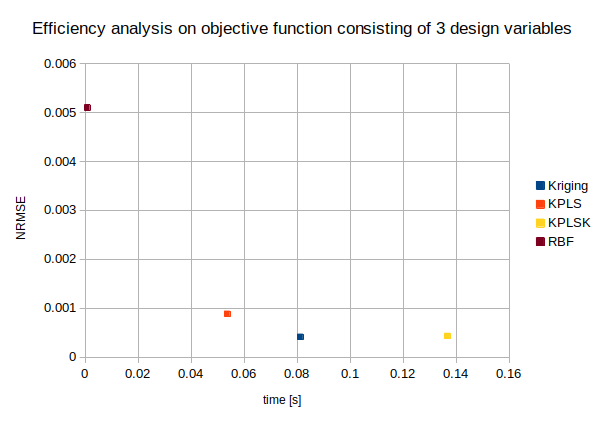
\includegraphics[width=0.75\textwidth]{Figure_47}
    \caption{Efficiency analysis on eq. \ref{pseudo_aircraft}}
\end{figure}

\begin{figure}[h!]
    \centering
    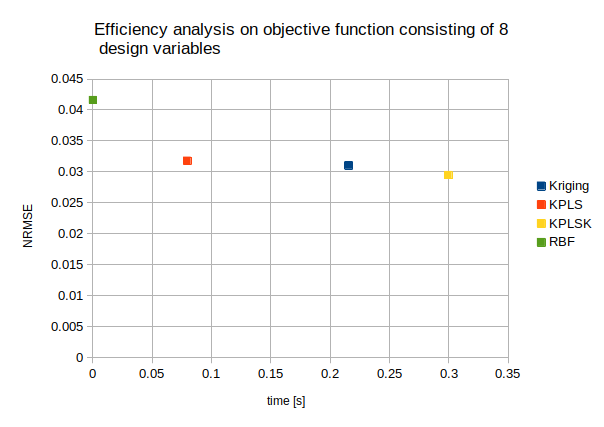
\includegraphics[width=0.75\textwidth]{Figure_38}
    \caption{Efficiency analysis on eq. 
    \ref{aircraft2}}
\end{figure}

\newpage
%-----------------------------------------------------------------

\chapter{SMT}

\section{DoE techniques in SMT}
The implementation of the sampling process is facilitated by a 
Python-based, open-source software, called SMT. The DoE sampling 
techniques available in SMT are implemented in the 3D design space 
defined by the bounds of the 3 design variables in equation 
\ref{pseudo_aircraft}, i.e. $\vec{β}= [β_{1}, β_{2}, β_{3}] 
\!= \![S,N_{z},AR]$, where $120 < S < 170$, $2 < N_{z} < 6$ and 
$6 < AR < 11$. The constructed designs consist of $n_{doe} \!= 
\!40$ samples; the corresponding Python scripts are presented 
subsequently.

\begin{itemize}
\item \textbf{Random sampling} \\
The creation of a randomly generated design can be accomplished 
in SMT by executing a Python script with the following form:

\begin{lstlisting}[language = Python, caption = Implementation of 
Random sampling]
import numpy as np
from smt.sampling_methods import Random

ndoe = 40 #number of sample points
betalimits = np.array([[120.0,170.0], [2.0,6.0], [6.0,11.0]])
sampling = Random(xlimits = betalimits)   
beta = sampling(ndoe)
\end{lstlisting}

\item \textbf{Latin Hypercube Sampling (LHS)} \\
LHS is a stratified sampling approach with the restriction that each 
of the input variables has its range well sampled following a 
probability distribution. In SMT, the creation of a LHD is 
performed by executing a Python script as such: 

\begin{lstlisting}[language = Python, caption = Implementation of 
LHS]
import numpy as np
from smt.sampling_methods import LHS

ndoe = 40 #number of sample points
betalimits = np.array([[120.0,170.0], [2.0,6.0], [6.0,11.0]])
sampling = LHS(xlimits = betalimits, criterion = 'ese')   
beta = sampling(ndoe)
\end{lstlisting}

The Python function LHS assumes various input values depending 
on the scheme used to construct the LHD. The process of 
constructing such a design is facilitated by PyDOE\cite{pyDOE}, 
where the construction criterion is denoted by '\textit{c}',
'\textit{m}', '\textit{cm}', '\textit{corr}' and '\textit{ese}'
to refer to Centered, Maximin, Maximin Centered, Maxent and ESE 
LHD, respectively, as depicted in the following script:

\begin{lstlisting}[language = Python, caption = Various 
construction criteria]
import numpy as np
from smt.sampling_methods import LHS

ndoe = 40 #number of sample points
betalimits = np.array([[120.0,170.0], [2.0,6.0], [6.0,11.0]])
crit = ['c', 'm', 'cm', 'corr', 'ese']
i = int(input('Define criterion between 0 and 4:'))
sampling = LHS(xlimits = betalimits, criterion = crit[i])
beta = sampling(ndoe)   
\end{lstlisting}

In SMT, the LHDs can be further optimized by expanding the initial 
design by a multiple of the initial number of sample points. 
The expanded design is implemented by setting the parameter 
\textit{method} equal to either '\textit{basic}' or 
'\textit{ese}'. The former applies to centered, maximin, centered 
maximin and entropy LHDs, while the latter to ESE LHDs. The 
process of creating expanded LHDs is performed via the use of
a Python script of the following format:

\begin{lstlisting}[language = Python, caption = Expanded LHD]
import numpy as np
from smt.sampling_methods import LHS

#Initial LHD
ndoe = 40 #number of sample points
betalimits=np.array([[120.0,170.0], [2.0,6.0], [6.0,11.0]])
sampling = LHS(xlimits = betalimits, criterion = 'ese', random_state = 1)
beta = sampling(ndoe)
#Expanded LHD
n_newdoe=ndoe #Points to be added
beta_new = sampling.expand_lhs(beta, n_newdoe, method = 'basic')
  
\end{lstlisting}

where \textit{random\_state} is a keyword argument that is used 
to control the Mersenne Twister pseudo-random number generator 
If the input value can be an integer between 0 and $2^{32}-1$, 
an array of integer values, or type $None$ that is the default 
setting. As long as the argument assumes the same input value, it
produces the same outcome and therefore this method is used for
reproducibility.

\item \textbf{Full Factorial} \\
Although this sampling method is referred to as Full Factorial 
in SMT documentation, it creates either Full or Fractional 
Factorial Designs and can be used by executing a Python script 
that resembles the following form:

\begin{lstlisting}[language = Python, caption = Implementation of 
Full Factorial sampling]
import numpy as np
from smt.sampling_methods import FullFactorial

ndoe = 40 #number of sample points
betalimits = np.array([[120.0,170.0], [2.0,6.0], [6.0,11.0]])
sampling = FullFactorial(xlimits = betalimits)   
beta = sampling(ndoe)
\end{lstlisting}

\end{itemize}


\newpage
%-------------------------------------------------------------


\section{Metamodel Training}

\begin{itemize}
\item \textbf{Kriging} \\
The four correlation functions in SMT are declared in the 
corresponding Python function as an additive parameter 
\textit{corr}, which is set to 'abs\_exp' (exponential), 
'squar\_exp' (Gaussian), 'matern52' and 'matern32', respectively. 
Additionally, it is possible to alternate between regression models 
by defining an extra input parameter in Python; that parameter is 
$poly$ and can be set to 'constant', 'linear' or 'quadratic', which 
corresponds to a constant, linear or quadratic model as the 
notation implies. The correlation parameters $θ \!\in \!\mathbb{R}
^{n_{β}}$ are computed via the maximum likelihood estimation of 
equation \ref{max_likelihood_fun}, which is minimized via the use 
of COBYLA algorithm  \cite{COBYLA}, provided by the open-source 
Python library sciPy\cite{scipy}. A typical Python script that 
performs the training of Kriging model has the following form:

\begin{lstlisting}[language = Python, caption = Training of Kriging model with noise-free observations via SMT]
import numpy as np
from smt.surrogate_models import KPLS, KRG, KPLSK, RBF

.... 
ndim = 3 #number of problem dimensions
list0 = ['constant', 'linear', 'quadratic']
list1 = ['abs_exp', 'squar_exp', 'matern52', 'matern32']    

polynomial = int(input('Define regression model between 0 and 3:'))
correlation = int(input('Define correlation function between 0 and 4:'))
th_range = np.array(([1e-8, 1e+3]))
t = KRG(theta0 = [1e-2]*ndim, theta_bounds = th_range, poly = list0[polynomial], corr = list1[correlation], eval_noise = False)     
t.set_training_values(beta,F)
t.train()
\end{lstlisting}

In order for the Python to account for 
the existing noise the parameter \textit{eval\_noise} must be set 
to 'True'. In addition, the lower bound for nugget must be 
defined by using the parameter \textit{nugget} and the value 
of the initial noise parameters must be defined via the 
parameter \textit{noise0}. The default values of 
\textit{nugget} and \textit{noise0} are $2.220446049250313 
\cdot 10^{-14}$ and $0$ for each design variable, 
respectively.

\begin{lstlisting}[language = Python, caption = Training of Kriging model with noisy observations via SMT]
import numpy as np
from smt.surrogate_models import KRG

.... 
ndim = 3 #number of problem dimensions
th_range = np.array(([1e-8, 1e+3]))
t = KRG(theta0 = [1e-2]*ndim, theta_bounds = th_range, poly = 'constant', corr = 'squar_exp', eval_noise = True, noise0 = [1e-2])     
t.set_training_values(beta,F)
t.train()
\end{lstlisting}

\newpage
%------------------------------------------------------------------


\item \textbf{KPLS} \\
The number of principal components in SMT is declared 
in the corresponding Python function via the additive 
parameter \textit{n\_comp}. All the other parameters are
defined similarly to Kriging model.

\begin{lstlisting}[language = Python, caption = Training of KPLS model with noisy observations via SMT]
import numpy as np
from smt.surrogate_models import KPLS

.... 
n_com = 2 #number of principal components
th_range = np.array(([1e-8, 1e+3]))
t = KPLS(n_comp = n_com, theta0 = [1e-2]*n_com, theta_bounds = th_range, poly = 'constant', corr = 'squar_exp')    
t.set_training_values(beta,F)
t.train()
\end{lstlisting}

\item \textbf{KPLSK} \\
All the necessary parameters in 
KPLSK model are declared in Python script similarly to 
KPLS and Kriging.

\begin{lstlisting}[language = Python, caption = Training of KPLSK model with noisy observations via SMT]
import numpy as np
from smt.surrogate_models import KPLSK

.... 
n_com = 2 #number of principal components
th_range = np.array(([1e-8, 1e+3]))
t = KPLSK(n_comp = n_com, theta0 = [1e-2]*n_com, theta_bounds = th_range, poly = 'constant', corr = 'squar_exp')    
t.set_training_values(beta,F)
t.train()
\end{lstlisting}

\item \textbf{RBF} \\
In SMT, the degree and the existence of polynomials can be 
determined by modifying the value of the Python parameter 
\textit{poly\_degree}. Consequently, a value of -1, 0 or 1 is used 
to denote the absence of a polynomial trend, a constant trend and 
a linear trend respectively. If no polynomial trend is used, i.e. 
$poly\_degree \!= \!-1$, multivariate RBF interpolation is 
performed by solving the linear system described by equations 
\ref{RBF_no_poly} and \ref{RBF_no_poly_matrix}. If however 
$poly\_degree \!= \!1$, then RBF interpolation is performed by solving the linear system described by eq. 
\ref{RBF_poly_linear_matrix}.

\begin{lstlisting}[language = Python, caption = Training of KPLSK model with noisy observations via SMT]
import numpy as np
from smt.surrogate_models import RBF

.... 
t = RBF(d0 = 100, poly_degree = 1)   
t.set_training_values(beta,F)
t.train()
\end{lstlisting}

\end{itemize}



\newpage
%-------------------------------------------------------------




\chapter{EASY}
\label{appendix:EASY}
In order to gain a better grasp of how the communication 
channel between SMT and EASY\cite{EASY} software is 
established, first, it is important to analyze the way 
EASY optimization software works. 

\begin{itemize}
\item \textbf{EASY and EAs}
\end{itemize}
 
In EASY menu, the parameters of the optimization and 
both the bounds and the codification of the design variables 
can be modified. The evolutionary process via the use of EASY 
is performed as follows:

\begin{enumerate}
\item To perform an evaluation EASY writes and saves an 
ASCII text file \textit{task.dat} that consists of $n_{β}+1$ 
lines. The first line corresponds to the selected number of 
design variables $n_{β}$, while the remaining lines contain 
the values of each design variable and are listed according 
to the sequence declared by the user in EASY.  

\item EASY executes the batch file \textit{task.bat} and then
halts all other processes until \textit{task.bat} is 
finished. In EASY, this batch file is responsible for 
executing all processes responsible for the evaluation of 
candidate solutions (EAs-2). A typical \textit{task.bat} has the 
following structure:

\begin{lstlisting}[language = command.com, caption = Structure of 
\textit{task.bat} file]
@echo off
erase results.dat
preprocessor.exe > nul 
evaluation.exe > nul 
postprocessor.exe > nul
\end{lstlisting}

where @echo off in \textit{Windows} OS, prevents the 
the system terminal from printing any optimization-related 
results. The $> nul$ command uses as output of the respective 
executable process the temporary file nul. 

\item After the results of the previous run have been deleted, 
\textit{preprocessor.exe} is executed. This executable is 
responsible for reading \textit{task.bat} file and transforms
the collected data in a readable format for the next process.

\newpage
%---------------------------------------------------------------


\item The evaluation of any untried candidate solution $\vec{β} 
\!\in \!P_{λ}^{g} \!\subset \!\mathbb{R}^{n_{β}}$ is performed 
via the execution of process \textit{evaluation.exe} that contains 
the problem-specific model, in most cases a CFD tool.

\item The value of each objective and design variable value is 
then written in a ASCII text file \textit{results.dat}; each line
of that file contains a single value.

\item Subsequently, \textit{postprocessor.exe} is executed. 
This executable reads the output of \textit{evaluation.exe}, 
i.e. \textit{results.dat} file, and allows the user to denote 
the necessary objectives and constraints of the optimization via 
the creation of \textit{task.res} and \textit{task.cns}, 
respectively.

\item After \textit{task.bat} has finished, EASY expects to 
read a plain ASCII text file, \textit{task.res}, which 
contains as many lines as the number of objectives. Each line 
of that file contains the value of the corresponding 
objective. 

\item Most optimization problems are confronted w.r.t. 
a set of imposed constraints. In EASY, these constraints 
are declared in a plain ASCII text file, 
\textit{task.cns}, which contains as many
lines as the number of constraints imposed.

\end{enumerate}